\documentclass[12pt,letterpaper]{article}
\usepackage{preamble}
\usepackage{graphicx}
\usepackage{subcaption}

%%%%%%%%%%%%%%%%%%%%%%%%%%%%%%%%%%%%%%%%%%
%%%% Edit These for yourself
%%%%%%%%%%%%%%%%%%%%%%%%%%%%%%%%%%%%%%%%%%
\newcommand\course{}
\newcommand\hwnumber{1}
\newcommand\userID{Marina E. Almenzar}

\begin{document}
\section*{Programming Exercise 1}
\subsection*{Regression Task}
Choose a regression dataset and apply linear regression on a random subset of the training set of increasing size. You should select training sets that include more and more data points.
\begin{enumerate}[leftmargin=!,labelindent=5pt]
    \item Plot the approximation error (square loss) on the training set as a function of the number of samples $N$, i.e., data points in the training set.
        \begin{figure}[H]
            \centering
            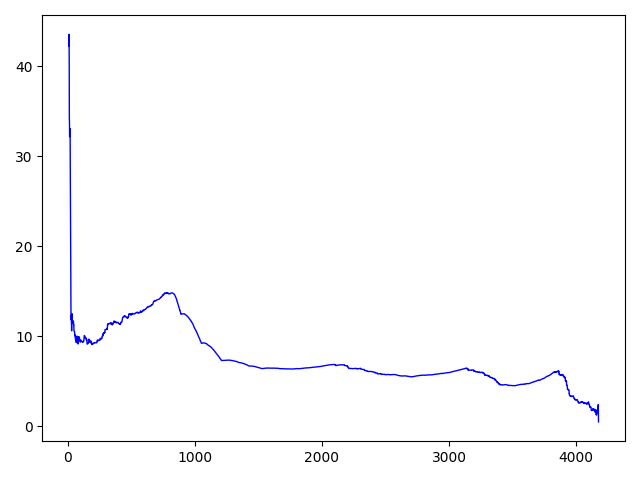
\includegraphics[width=15cm]{images/error.jpg}
            \caption{Approximation error (square loss) on the training set as a function of the number of samples $N$ for the \textit{abalone.txt} example}
            \label{fig:1}
        \end{figure}
    \newpage
    \item Plot the cpu-time as a function of $N$.
        \begin{figure}[H]
            \centering
            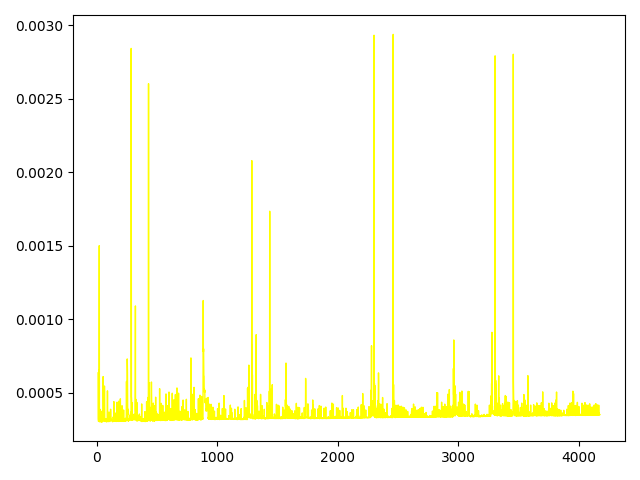
\includegraphics[width=15cm]{images/time.jpg}
            \caption{CPU-time as a function of the number of samples $N$ for the \textit{abalone.txt} example}
            \label{fig:1}
        \end{figure}
        
    \newpage
    \item Explain in detail the behaviour of both curves: what is the trend you observe? does it stabilize? why?
    
    The approximation error (square loss) decreases when $N$ increases and stabilizes, because when $N$ increases we are actually increasing the training dataset, and it allows a better fit of the model.
    The CPU-time does not stabilize.
        
        
    \newpage
    \item Explore how the learned weights change as a function of $N$. For this, you can make separate stem plots for several values of $N$. Can you find an interpretation for the learned weights?

        \begin{figure}[H]
        \begin{subfigure}{0.3\textwidth}
        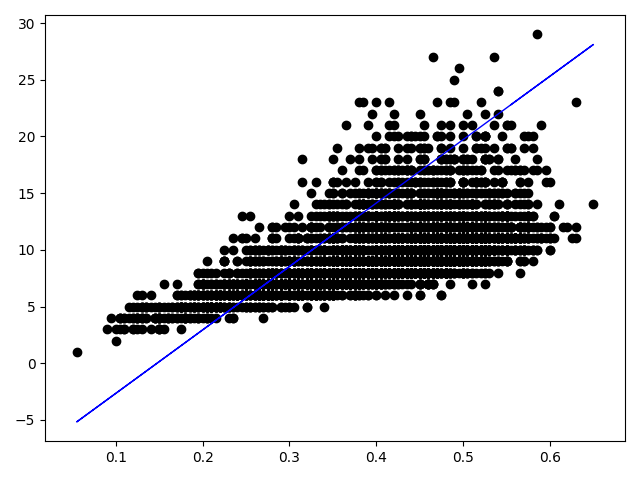
\includegraphics[width=5cm]{images/M10.jpg} 
        \caption{$N = 10$}
        \label{fig:subim4}
        \end{subfigure}
        \begin{subfigure}{0.3\textwidth}
        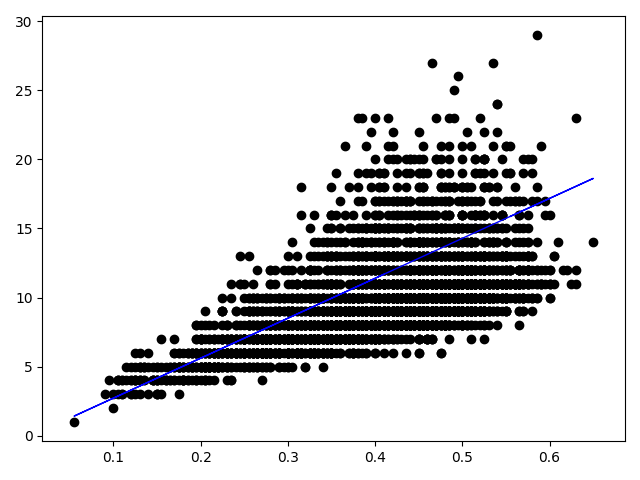
\includegraphics[width=5cm]{images/M50.jpg}
        \caption{$N = 50$}
        \label{fig:subim5}
        \end{subfigure}
        \begin{subfigure}{0.3\textwidth}
        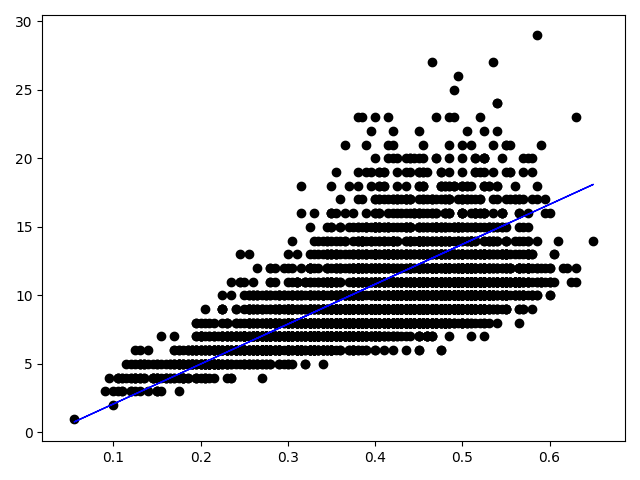
\includegraphics[width=5cm]{images/M100.jpg}
        \caption{$N = 100$}
        \label{fig:subim6}
        \end{subfigure}
        
        \begin{subfigure}{0.3\textwidth}
        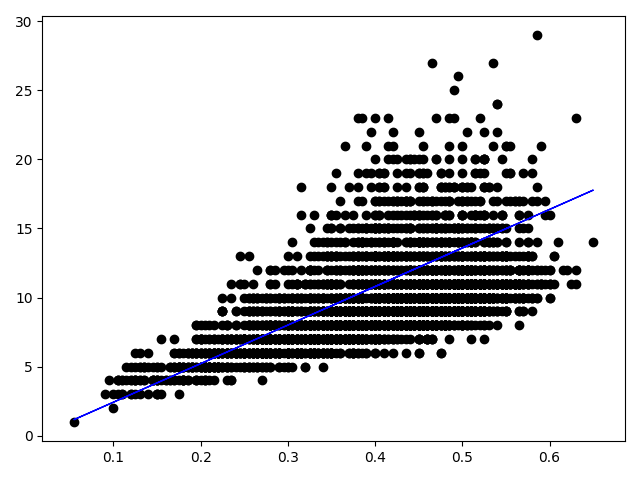
\includegraphics[width=5cm]{images/M200.jpg} 
        \caption{$N = 200$}
        \label{fig:subim4}
        \end{subfigure}
        \begin{subfigure}{0.3\textwidth}
        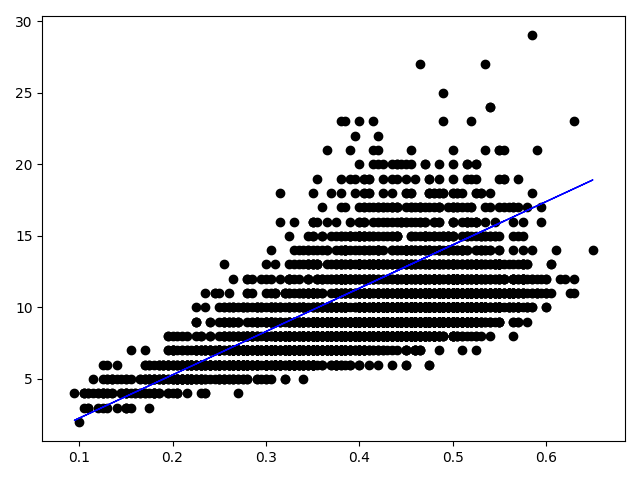
\includegraphics[width=5cm]{images/M400.jpg}
        \caption{$N = 400$}
        \label{fig:subim5}
        \end{subfigure}
        \begin{subfigure}{0.3\textwidth}
        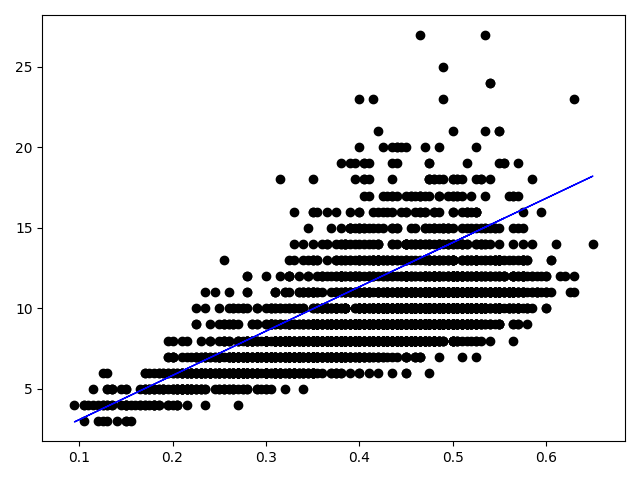
\includegraphics[width=5cm]{images/M1000.jpg}
        \caption{$N = 1000$}
        \label{fig:subim6}
        \end{subfigure}
        
        \begin{subfigure}{0.3\textwidth}
        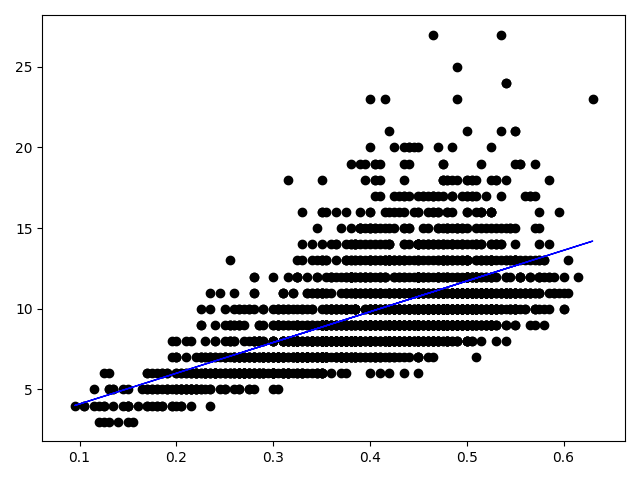
\includegraphics[width=5cm]{images/M2000.jpg} 
        \caption{$N = 2000$}
        \label{fig:subim4}
        \end{subfigure}
        \begin{subfigure}{0.3\textwidth}
        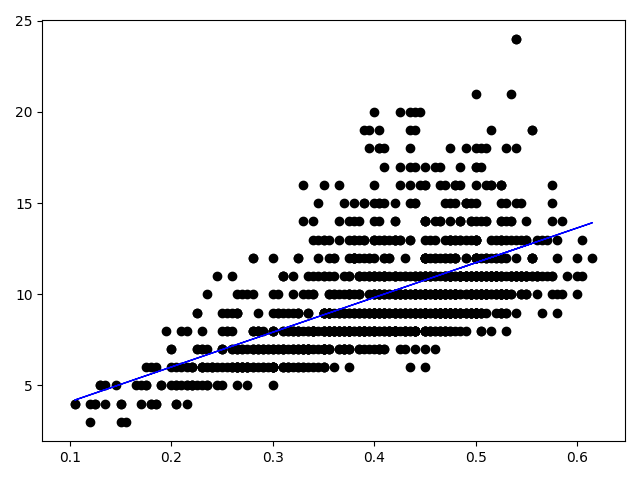
\includegraphics[width=5cm]{images/M3000.jpg}
        \caption{$N = 3000$}
        \label{fig:subim5}
        \end{subfigure}
        \begin{subfigure}{0.3\textwidth}
        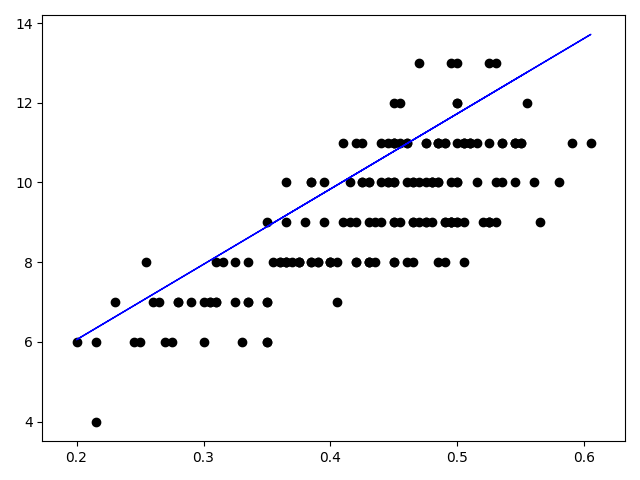
\includegraphics[width=5cm]{images/M4000.jpg}
        \caption{$N = 4000$}
        \label{fig:subim6}
        \end{subfigure}
        \caption{Separate stem plots for several values of $N$,  for the \textit{abalone.txt} example. Black points are the  test set and the blue line is the prediction of the linear regression model, fit with the training set of  size $N$}
        \end{figure}
\end{enumerate}
\newpage
\subsection*{Classification Task}
Choose a classification dataset and apply logistic regression. Repeat the previous four steps using as error the mean accuracy.

\begin{enumerate}[leftmargin=!,labelindent=5pt]
    \item Plot the mean accuracy on the training set as a function of the number of samples $N$, i.e., data points in the training set.
        \begin{figure}[H]
            \centering
            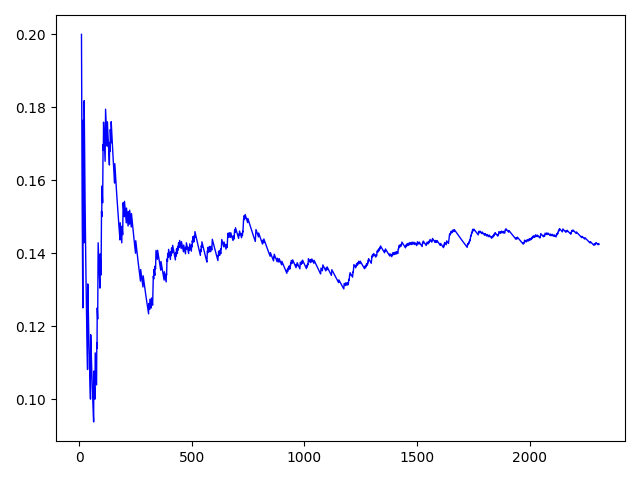
\includegraphics[width=15cm]{images/log_accurate.jpg}
            \caption{Mean accuracy on the training set as a function of the number of samples $N$, for the \textit{segment.scale.txt} example}
            \label{fig:1}
        \end{figure}
    \newpage
    \item Plot the cpu-time as a function of $N$.
        \begin{figure}[H]
            \centering
            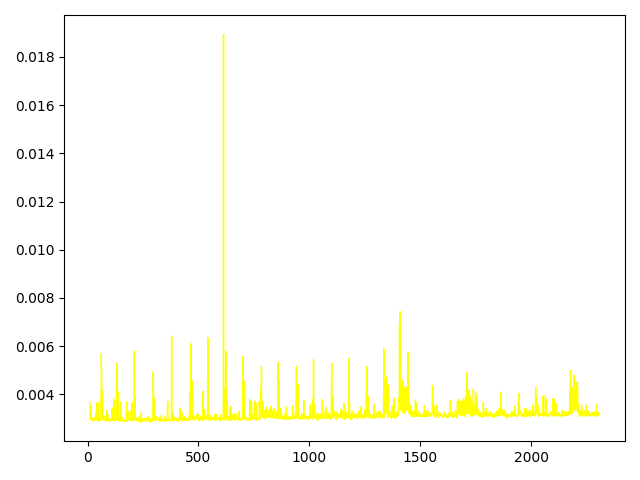
\includegraphics[width=15cm]{images/log_time.jpg}
            \caption{CPU-time as a function of the number of samples $N$, for the \textit{segment.scale.txt} example}
            \label{fig:1}
        \end{figure}
    \newpage
    \item Explore how the learned weights change as a function of $N$. For this, you can make separate stem plots for several values of $N$. Can you find an interpretation for the learned weights?
    \begin{figure}[H]
        \begin{subfigure}{0.3\textwidth}
        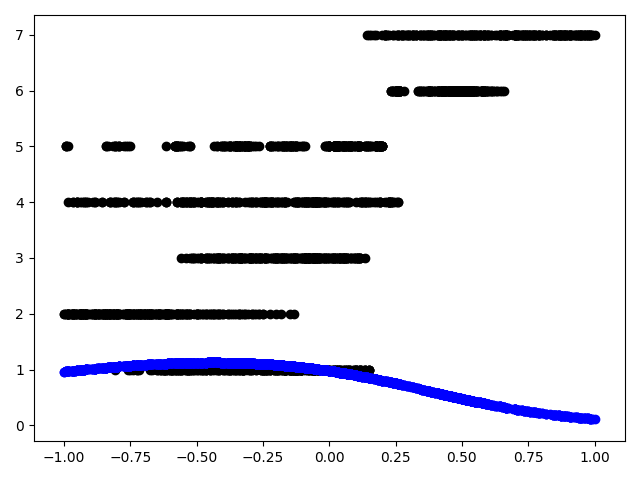
\includegraphics[width=5cm]{images/log100.jpg} 
        \caption{$N = 100$}
        \label{fig:subim4}
        \end{subfigure}
        \begin{subfigure}{0.3\textwidth}
        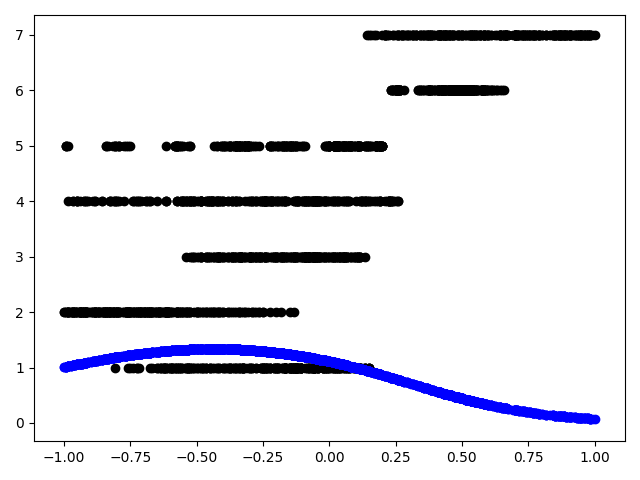
\includegraphics[width=5cm]{images/log150.jpg}
        \caption{$N = 150$}
        \label{fig:subim5}
        \end{subfigure}
        \begin{subfigure}{0.3\textwidth}
        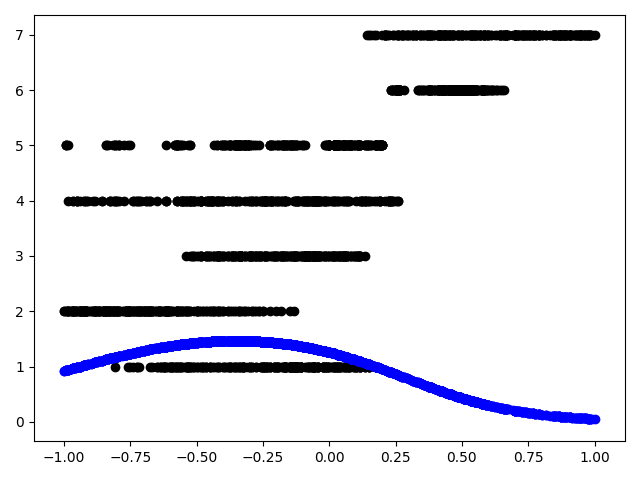
\includegraphics[width=5cm]{images/log200.jpg}
        \caption{$N = 200$}
        \label{fig:subim6}
        \end{subfigure}
        
        \begin{subfigure}{0.3\textwidth}
        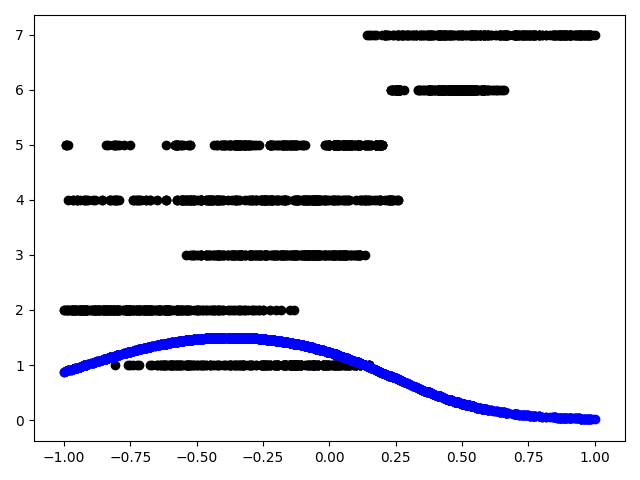
\includegraphics[width=5cm]{images/log300.jpg} 
        \caption{$N = 300$}
        \label{fig:subim4}
        \end{subfigure}
        \begin{subfigure}{0.3\textwidth}
        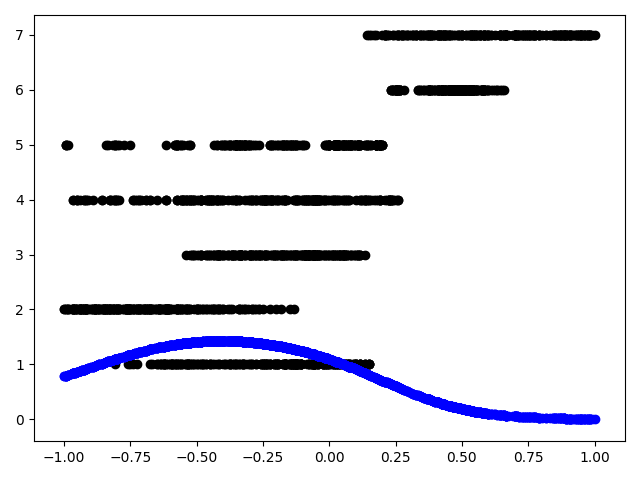
\includegraphics[width=5cm]{images/log400.jpg}
        \caption{$N = 400$}
        \label{fig:subim5}
        \end{subfigure}
        \begin{subfigure}{0.3\textwidth}
        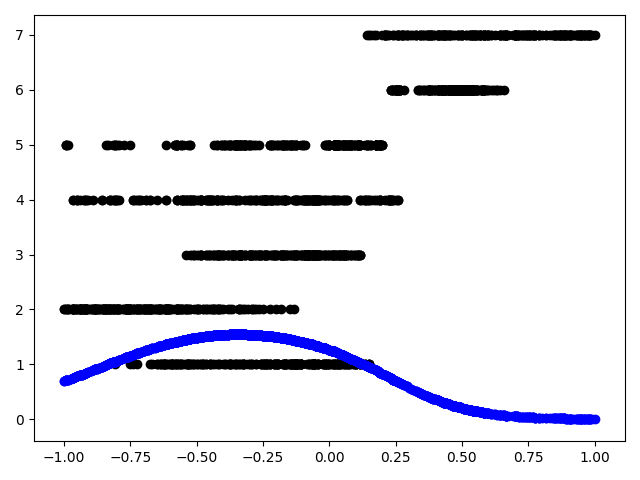
\includegraphics[width=5cm]{images/log500.jpg}
        \caption{$N =500$}
        \label{fig:subim6}
        \end{subfigure}
        
        \begin{subfigure}{0.3\textwidth}
        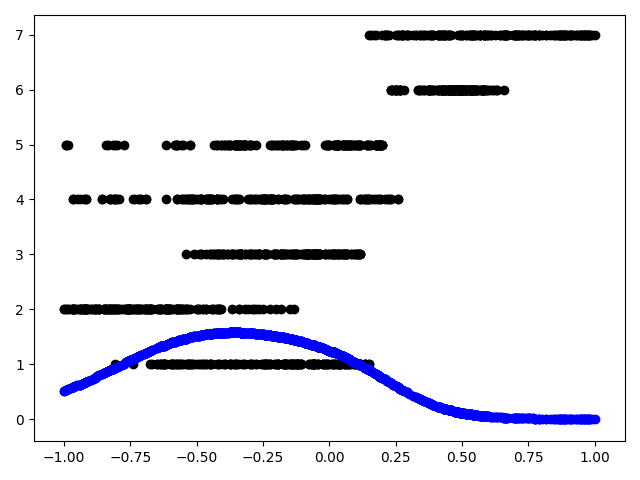
\includegraphics[width=5cm]{images/log1000.jpg} 
        \caption{$N = 1000$}
        \label{fig:subim4}
        \end{subfigure}
        \begin{subfigure}{0.3\textwidth}
        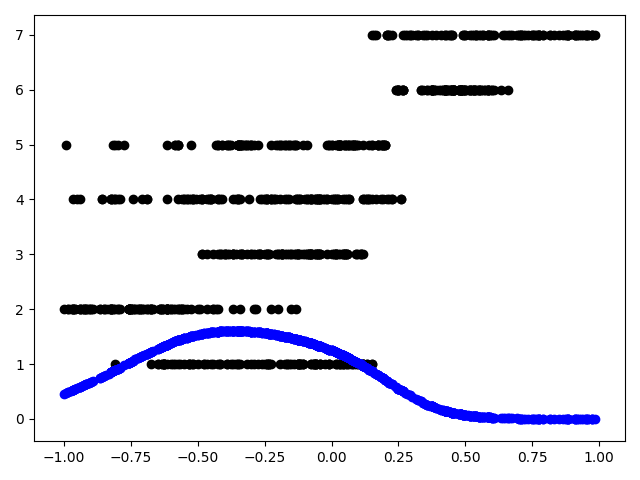
\includegraphics[width=5cm]{images/log2000.jpg}
        \caption{$N = 2000$}
        \label{fig:subim5}
        \end{subfigure}
        \begin{subfigure}{0.3\textwidth}
        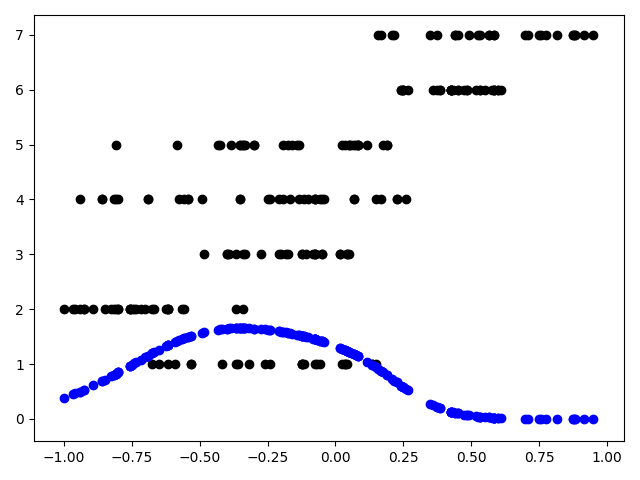
\includegraphics[width=5cm]{images/log2100.jpg}
        \caption{$N =2100$}
        \label{fig:subim6}
        \end{subfigure}
    \caption{Blue points are the probability of which the data belong to class 2, deduced with the logistic regression model, fit with the training set of  size $N$. The figures are separate stem plots for several values of $N$,  for the \textit{segment.scale.txt} example}
    \end{figure}
\end{enumerate}
\end{document}
